% !TeX encoding = UTF-8
% !BIB TS-program = XeLaTex
%% abtex2-modelo-slides.tex, v-1.0 gfabinhomat
%% Copyright 2012-<COPYRIGHT_YEAR> by abnTeX2 group at http://www.abntex.net.br/ 
%%
%% This work may be distributed and/or modified under the
%% conditions of the LaTeX Project Public License, either version 1.3
%% of this license or (at your option) any later version.
%% The latest version of this license is in
%%   http://www.latex-project.org/lppl.txt
%% and version 1.3 or later is part of all distributions of LaTeX
%% version 2005/12/01 or later.
%%
%% This work has the LPPL maintenance status `maintained'.
%% 
%% The Current Maintainer of this work is Fábio Rodrigues Silva, 
%% member of abnTeX2 team, led by Lauro César Araujo. 
%% Further information are available on 
%% http://www.abntex.net.br/
%%
%% This work consists of the files slides.tex, 
%% abntex2-modelo-references.bib and abntex2-modelo-marca.pdf
%%
%% Modelo desenvolvido por Fábio Rodrigues Silva (gfabinhomat@gmail.com)
%% Mais informações podem ser obtidas no guia do usuário Beamer 
%% (http://linorg.usp.br/CTAN/macros/latex/contrib/beamer/doc/beameruserguide.pdf)
%% Informações rápidas podem ser acessadas em http://en.wikibooks.org/wiki/LaTeX/Presentations
%%
%% Alterações no modelo - por Danny Tonidandel (tonidandel@gmail.com)
%% 1) Cores do sistema, sobretudo na página de título, com logos das instituições;
%% 2) pacotes para compilação a partir do XeLaTeX e bibliografias reduzidas (ibid., op.cit. etc.) em notas de rodapé, estilo biblatex-abnt-ibid ou estilo abnt com notas explicativas;
%% 3) Adequações para url - NBR6023-2018



% Apresentações em widescreen. Outros valores possíveis: 1610, 149, 54, 43 e 32.
% Por padrão, as apresentações são no formato 4:3 (sem o aspectratio).
\documentclass[aspectratio=169]{beamer}	 	

\usetheme{Pittsburgh}
\usecolortheme{default}
\usefonttheme[onlymath]{serif}			% para fontes matemáticas
% Enconte mais temas e cores em http://www.hartwork.org/beamer-theme-matrix/ 
% Veja também http://deic.uab.es/~iblanes/beamer_gallery/index.html

% Customizações de Cores: fg significa cor do texto e bg é cor do fundo
\definecolor{coolblack}{rgb}{0.0, 0.18, 0.39} % define cor coolblack
\definecolor{cornellred}{rgb}{0.7, 0.11, 0.11} % define cor cornellred
\definecolor{darkelectricblue}{rgb}{0.33, 0.41, 0.47} % define cor darkelectricblue
%% Para definir mais cores, visite https://latexcolor.com/

\setbeamercolor{normal text}{fg=black}
\setbeamercolor{alerted text}{fg=cornellred}
\setbeamercolor{author}{fg=cornellred}
\setbeamercolor{institute}{fg=coolblack}
\setbeamercolor{date}{fg=darkelectricblue}
\setbeamercolor{frametitle}{fg=coolblack}
\setbeamercolor{framesubtitle}{fg=cornellred}
\setbeamercolor{block title}{bg=darkelectricblue, fg=white}		%Cor do título
\setbeamercolor{block body}{bg=lightgray, fg=darkgray}	%Cor do texto (bg= fundo; fg=texto)

% ---
% PACOTES
% ---
%\usepackage[alf]{abntex2cite}		% Citações padrão ABNT
\usepackage[backend=biber,
style=abnt,
sccite,
citecount,
ittitles,
scbib,
justify,
noslsn,
repeatfields]{biblatex} % Citações padrão ABNT com estilo biblatex-abnt

\addbibresource{referencias.bib}
\usepackage{relsize} % precisa ser readicionado por que senão o comando \part não funciona no biblatex.  
\usepackage[brazil]{babel}		% Idioma do documento em português
\usepackage{color}			% Controle das cores
\usepackage{amsmath,amssymb,unicode-math} % segundo informacoes, o pacote unicode-math é mais adequado para o compilador xelatex, ao invés do amsfonts
%\usepackage[T1]{fontenc}		% Selecao de codigos de fonte.
\usepackage{graphicx}			% Inclusão de gráficos
%\usepackage[utf8]{inputenc}		% Codificacao do documento (conversão automática dos acentos)
%\usepackage{txfonts}			% Fontes virtuais
\usepackage{csquotes}

% --- Adequacao ao estilo abnt (2018) - formata campo url
\DeclareFieldFormat{url}{\bibstring{urlfrom}\addcolon\addspace \url{#1}}%

% --- Informações do documento ---
\title{Um título interessante}
\author{Fulanx de tal}
\institute{Dissertação (mestrado)
	\par
	Orientador: Profa. Mary B. Hesse, PhD.
	    \par
	    Coorientador: Prof. Thomas Kuhn, PhD. 
    	}
\date{\small{\today}}
% ---

% ----------------- INÍCIO DO DOCUMENTO --------------------------------------
\begin{document}

% ----------------- NOVO SLIDE -- CAPA --------------------------------
\begin{frame}

\begin{minipage}{1\linewidth}
  \centering
  \begin{tabular}{ccc}
    \begin{tabular}{c}
      \includegraphics[width=1.5cm]{figuras/logo-ufmg.pdf} 
    \end{tabular}
    &
    \begin{tabular}{c}
      \textbf{Universidade Federal de Minas Gerais} \\ \textbf{Programa de Pós-Graduação em Engenharia Elétrica}
    \end{tabular}
	&
  \begin{tabular}{c}
	\includegraphics[width=1.5cm]{figuras/logo-ppgee.pdf}
\end{tabular}
  \end{tabular}
\end{minipage}

\titlepage % imprime dados como título e autor

\end{frame}

% ----------------- NOVO SLIDE --------------------------------
\begin{frame}{Sumário}
\tableofcontents
\end{frame}

% ----------------- NOVO SLIDE --------------------------------
\section{Telegrafia}

%% ----------------- NOVO SLIDE --------------------------------
\begin{frame}{Analogia Matemática}
\begin{minipage}{0.5\textwidth}
	\begin{figure}[hbtp]
		\centering
		\includegraphics[scale=0.2]{figuras/figura4-oliver-portrait.pdf}
		\caption{Oliver Heaviside (1850-1925)} 
	\end{figure}
\end{minipage}
\begin{minipage}{0.47\textwidth}
Em (1893): $$\mbox{se}\; \; p \cdot f(t) = \frac{df(t)}{dt} \Rightarrow \frac{1}{p} \cdot f(t) = \int \limits_{0}^{t} f(\tau)d \tau \,.$$
%		\begin{eqnarray}
%			\mbox{se}\; \; p \cdot f(t) &=& \frac{df(t)}{dt} \,, \nonumber \\
%			\mbox{ent{\~a}o} \, \, \frac{1}{p} \cdot f(t) &=& \int \limits_{0}^{t} f(\tau)d \tau \,. \nonumber\\ 
%			{p}^{-1} \cdot H(t) & = & \int \limits_{0}^{t} H(\tau)d \tau  = t  \nonumber \\
%			{p}^{-2} \cdot H(t) & = & {p}^{-1} \cdot {p}^{-1} \cdot H(t) = \frac{t^2}{2!} \nonumber \\
%			& \vdots & \nonumber
%			{p}^{-n} \cdot H(t) & = & \frac{t^n}{n!} \;. \nonumber \label{eq:operadorp}
%		\end{eqnarray}

		Antes disso, porém, (1876): $$\frac{\partial^{2} v}{\partial x^{2}} = kc\frac{\partial v}{\partial t} + sc\frac{\partial^{2} v}{\partial t^{2}}\,.$$
\end{minipage}
\end{frame}
%% ----------------- NOVO SLIDE --------------------------------

% ----------------- NOVO SLIDE --------------------------------
\begin{frame}
\begin{figure}
	\centering
	\includegraphics[scale=0.30]{figuras/dominio-publico/figura2-cabosubmarino1858.pdf}
	\caption{Primeiro cabo transatlântico funcional de telégrafos (1866), entre Valentia Bay, no Reino Unido, e Trinity Bay, Newfoundland, nas ex-colônias britânicas da América do Norte, atualmente Canadá.} 
	\label{fig:10} 
\end{figure}
\end{frame}
% ----------------- NOVO SLIDE --------------------------------

% ----------------- NOVO SLIDE --------------------------------
\begin{frame}{Telegrafia}
\begin{figure}[!hbt]
	\centering
	\includegraphics[scale=0.2]{figuras/palacio-de-cristal-1851.pdf}
	\caption{Palácio de Cristal, sede da ``Exposição Universal'' (1843-1851). Fonte: Read $\&$ Co. Engravers $\&$ Printers.} 
	\label{fig:501} 
\end{figure}
\end{frame}
% ----------------- NOVO SLIDE --------------------------------

% ----------------- NOVO SLIDE --------------------------------
\begin{frame}{Telegrafia}
\begin{figure}
	\centering
	\includegraphics[scale=0.14]{figuras/Chappesemaphore.pdf}
	\caption{Telégrafo semafórico de Claude Chappe (1792).} 
	\label{fig:502} 
\end{figure}
\end{frame}
% ----------------- NOVO SLIDE --------------------------------

% ----------------- NOVO SLIDE --------------------------------
\begin{frame}{Telegrafia}
\begin{figure}
	\centering
	\includegraphics[scale=0.2]{figuras/Gauss-Weber-Telegraph.jpg}
	\caption{Tel{\'e}grafo eletromecânico de Weber criado em 1833, inspirado no sistema de Chappe. Na imagem é possível observar Gauss à direita, no receptor, e Weber à esquerda, como operador.}
	\label{fig:504}
\end{figure}
\end{frame}
% ----------------- NOVO SLIDE --------------------------------

% ----------------- NOVO SLIDE --------------------------------
\begin{frame}{Telegrafia}
%\framesubtitle{Mas afinal, o que é um telégrafo elétrico?}
\begin{figure}
	\includegraphics[scale=0.4]{figuras/basset2.pdf}
\end{figure}
\end{frame}
% ----------------- NOVO SLIDE --------------------------------

% ----------------- NOVO SLIDE --------------------------------
\begin{frame}{Telegrafia}
\begin{figure}
\includegraphics[scale=0.8]{figuras/telegrafo.pdf}
\end{figure}
\end{frame}
% ----------------- NOVO SLIDE --------------------------------

% ----------------- NOVO SLIDE --------------------------------
\begin{frame}{Ferrovias e Telegrafia}
\begin{figure}
	\includegraphics[scale=0.22]{figuras/fig08.pdf}
	\caption{O telégrafo elétrico no imaginário popular (1845).}
	\label{fig:08}
\end{figure}
\end{frame}
% ----------------- NOVO SLIDE --------------------------------

% ----------------- NOVO SLIDE --------------------------------
\begin{frame}{Telegrafia como profissão}
\begin{minipage}{0.47\textwidth}
	\begin{itemize}
		\item[-] Quando a telegrafia começa a se tornar rotineira, o sonho de ``interligar'' os dois continentes começa a tomar forma;
		\item[-] São criadas as companhias \emph{Atlantic Telegraph Company (UK)} e \emph{New York, Newfoundland and London Telegraph Company (US)} (1852);
		\item[-] Mas problemas aparentemente insolúveis poderiam por em cheque a realização dessa empreitada. 
	\end{itemize}
\end{minipage}
\begin{minipage}{0.5\textwidth}
\begin{figure}
	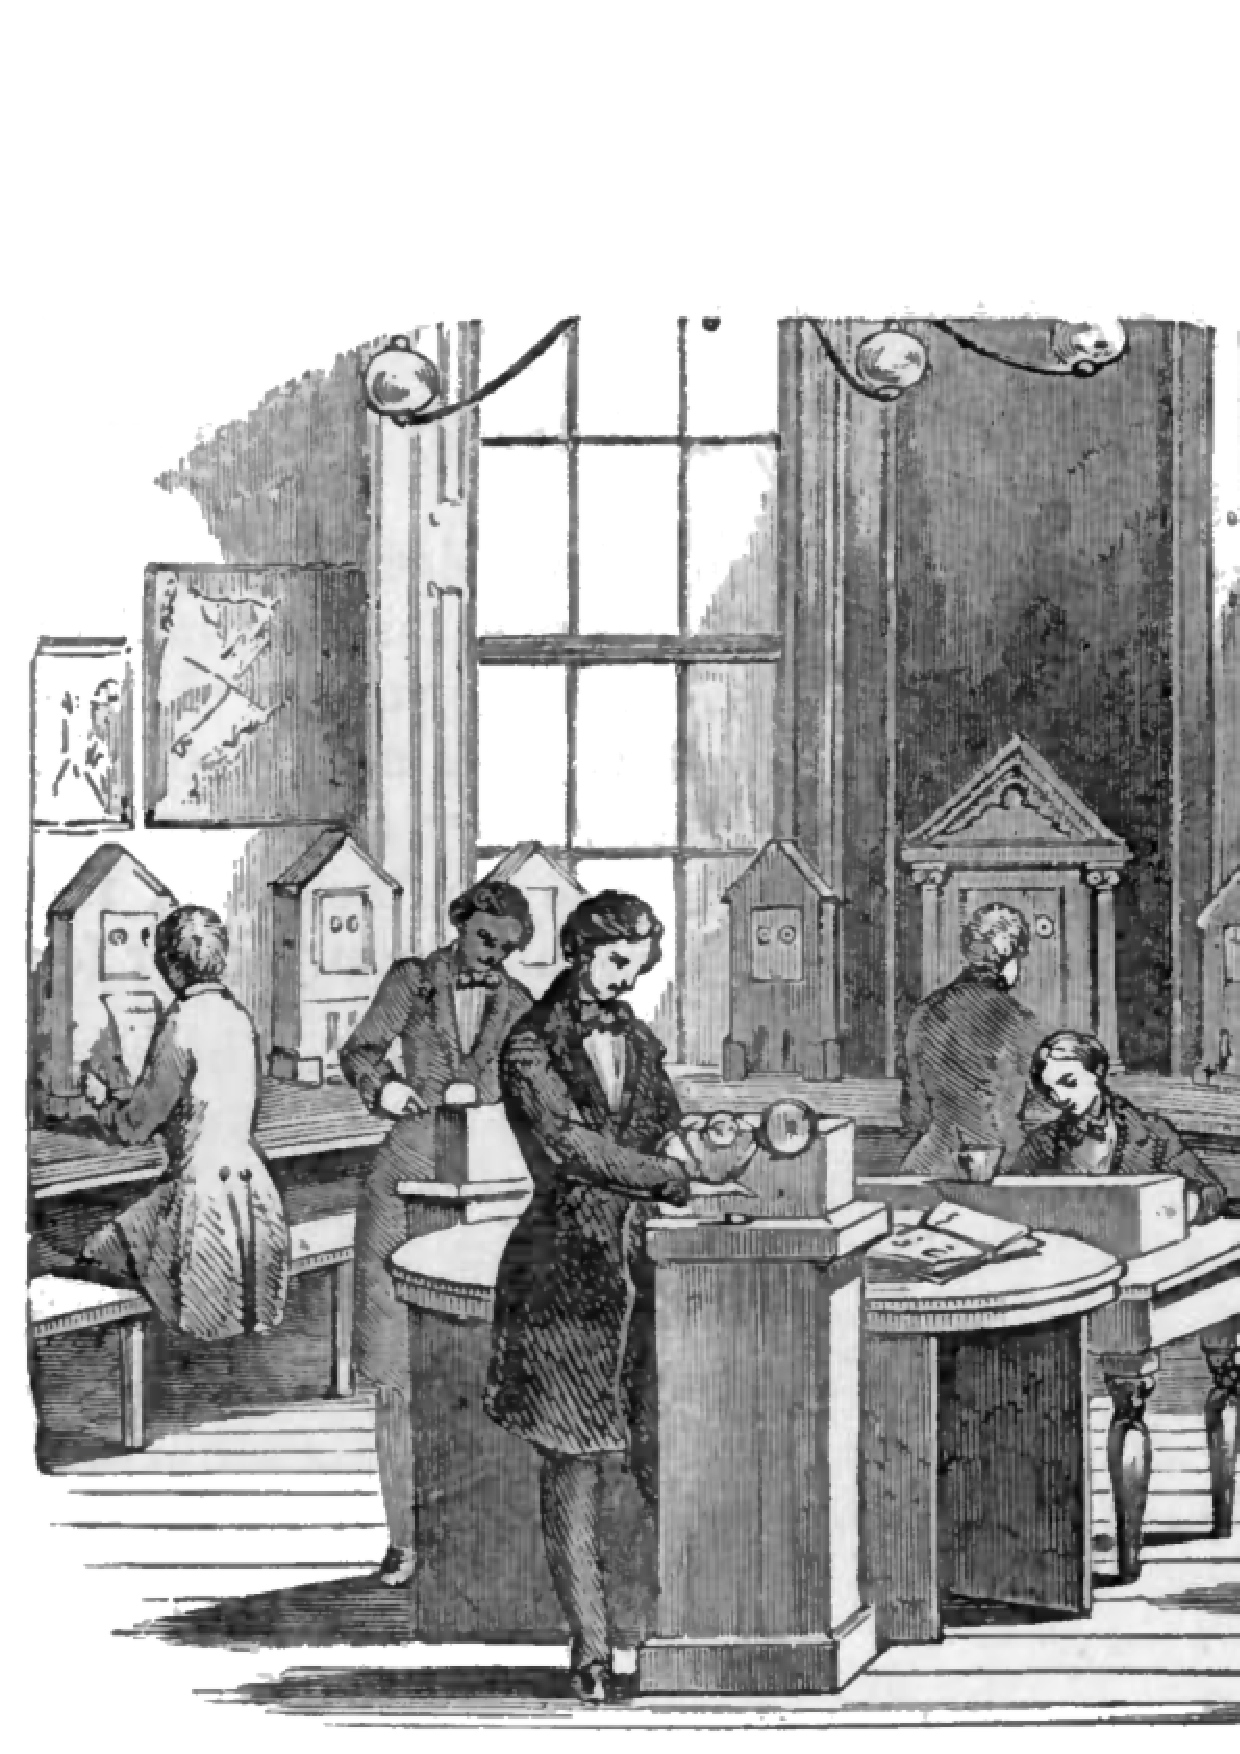
\includegraphics[scale=0.22]{figuras/fig09.pdf}
	\caption{Interior de um escritório de telegrafia.}
	\label{fig:09}
\end{figure}
\end{minipage}
\end{frame}
% ----------------- NOVO SLIDE --------------------------------


\section{O problema}
% ----------------- NOVO SLIDE --------------------------------
\begin{frame}{A charada elétrica}
\begin{minipage}{0.5\textwidth}
\centering
\begin{figure}[htbp]
	\includegraphics[scale=0.05]{figuras/thomson1859.pdf}
\end{figure}		
\begin{figure}[htbp]
	\includegraphics[scale=0.2]{figuras/geoge-stokes-1875.pdf}
\end{figure}		
\end{minipage}
\begin{minipage}{0.47\textwidth}
	\centering
\begin{figure}[htbp]
	\includegraphics[scale=0.2]{figuras/dominio-publico/locomotive.pdf}
	\caption{Locomotiva da Great Northern Railway, por volta de 1854. Fonte: Tony Hisgett (Wikimedia Commons)}
\end{figure}
\end{minipage}
\end{frame}
% ----------------- NOVO SLIDE --------------------------------

%% ----------------- NOVO SLIDE --------------------------------
%\begin{frame}{A charada elétrica}
%	\centering
%	\begin{figure}[htbp]
%		\includegraphics[scale=0.31]{figuras/dominio-publico/locomotive.pdf}
%		\caption{Great Northern Railway express locomotive, 1850-1922. Fonte: Tony Hisgett (Wikimedia Commons)}
%	\end{figure}
%\end{frame}
%% ----------------- NOVO SLIDE --------------------------------

% ----------------- NOVO SLIDE --------------------------------
\begin{frame}{A charada elétrica}
\begin{figure}[p]
	\centering
	\includegraphics[scale=0.25]{figuras/thomson-1854-primeiro-rascunho.eps}
%	\caption[A charada elétrica]{No verso da carta enviada por Stokes, Thomson busca uma solução rápida para a ``charada elétrica''.} 
	\label{fig:thomson1854-primeiro-rascunho} 
\end{figure}
\end{frame}
% ----------------- NOVO SLIDE --------------------------------

% ----------------- NOVO SLIDE --------------------------------
\begin{frame}{A charada elétrica}
	\begin{itemize}
		%	\item[-] A charada Elétrica;
		%\item[-] Ele havia definido os ``campos'' elétrico e magnético por meio da eq. da continuidade da hidrodinâmica, obtendo uma descrição geométrica para o movimento da eletricidade;\cite{tonidandel-et-al-2018}
		%\item[-] O aparato relacionava a ideia de ação à distância de uma força ao conceito de campo, dando o pontapé para uma teoria de campo para a eletrostática e, mais adiante, para a eletrodinâmica;
		\item[-] A partir daquela correspondência, em 1854,\cite{thomson1854} o jovem professor Thomson (1824-1907) propõe uma analogia para o ``movimento de eletricidade'' inspirada na teoria do calor de Fourier (1822),\cite{fourier1822} modelando o cabo como uma grande garrafa de Leyden;
		%\item[-] O projeto do Cabo Atlântico (1857-1866);
		%\item[-] Forte impacto econômico mundial;
		\item[-] A teoria era tautológica, mas contrariava tanto a metodologia de Fourier quanto a mentalidade pictórica da ciência Britânica;
	\end{itemize}
\end{frame}
% ----------------- NOVO SLIDE --------------------------------

% ----------------- NOVO SLIDE --------------------------------
\begin{frame}{A charada elétrica}
\begin{minipage}{0.47\textwidth}
\begin{figure}[hbtp]
	\centering
	\includegraphics[scale=0.3]{figuras/leydenjar2.pdf}
	\caption{Uma garrafa para o fluido elétrico.} 
	\label{fig:lydenjar2} 
\end{figure}
\end{minipage}
\begin{minipage}{0.5\textwidth}
\begin{figure}[htbp]
	\centering
	\includegraphics[scale=0.3]{figuras/cabo2.pdf}
	\caption{Geometria de um cabo submarino.} 
	\label{fig:cabo2} 
\end{figure}
\end{minipage}
\end{frame}
% ----------------- NOVO SLIDE --------------------------------

% ----------------- NOVO SLIDE --------------------------------
\begin{frame}{O problema}
\begin{minipage}{0.47\textwidth}
	\begin{itemize}
		\item[-] Por onde começar o estudo das analogias físicas?
		\item[-] A primeira teoria da propagação elétrica tem relação com antigas concepções de fluxo?
		\item[-] Hipótese: A analogia Eletricidade $\times$ Calor de W.T. estava refletida na ideia que ele e colaboradores nutriam acerca da continuidade; 
		\item[-] Necessidade de um grande recorte temporal.
	\end{itemize}
\end{minipage}
\begin{minipage}{0.5\textwidth}
	\begin{figure}
		\includegraphics[scale=0.3]{figuras/omnibuslondon.pdf}
	\end{figure}
\end{minipage}
\end{frame}
% ----------------- NOVO SLIDE --------------------------------

% ----------------- NOVO SLIDE --------------------------------
\begin{frame}{O problema}
\begin{itemize}
	\item[-] Quais as implicações da teoria para o estabelecimento da Engenharia Elétrica, que não esteve dissociada de outros ramos da atividade científica até o final do séc. XIX? 
	\item[-] É possível delimitar um Marco Zero para a Engenharia Elétrica?
	\item[-] Hipótese: O projeto do cabo, então sem precedentes, abriu um ``mercado'' não só para a Teoria de Campo do Eletromagnetismo, mas serviu de plataforma para toda uma estrutura baseada em eletricidade;
\end{itemize}
\end{frame}
% ----------------- NOVO SLIDE --------------------------------

% ----------------- NOVO SLIDE --------------------------------
\section{Metodologia e Organização}

\begin{frame}{Organização e metodologia}
\begin{minipage}{0.4\textwidth}
	\begin{figure}
		\centering
		\includegraphics[scale=0.2]{figuras/gota-dagua.pdf}
	\end{figure}
\end{minipage}
%\begin{minipage}{0.57\textwidth}
\begin{itemize}
	\item[-] Pierre Duhem:\cite{duhem1954} ``um experimento físico é sua interpretação teórica'';
	\item[-] Mary B. Hesse:\cite{hesse1962} ``Quaisquer fatos, históricos ou experimentais são produzidos à luz de determinada teoria'', i.e., analogia como fenômeno \emph{a priori}.
\end{itemize}
%\end{minipage}
\end{frame}
% ----------------- NOVO SLIDE --------------------------------

% ----------------- NOVO SLIDE --------------------------------
\begin{frame}{Estrutura de uma analogia}
``(...) Devemos, portanto, descobrir algum método de investigação que nos permita, a cada passo, desenvolver uma clara concepção física, sem nos comprometer com qualquer teoria fundada na ciência física da qual tal concepção foi retirada, de modo que não nos percamos na busca de sutilezas analíticas, nem ultrapassemos a linha da verdade levados por uma hipótese de especial predileção. Para se obter ideias físicas sem adotar uma teoria física, devemos nos familiarizar com a existência de analogias físicas. Analogia física, a meu ver, é aquela parcial similaridade entre as leis de uma ciência e aquelas de outra que faz cada qual ilustrar a outra. (...)''\cite{maxwell1855} 
\end{frame}
% ----------------- NOVO SLIDE --------------------------------

\begin{frame}{Estrutura de uma analogia}
\framesubtitle{Até agora...}
\begin{itemize}
	\item[-] Científica ou de síntese: materialização de uma identidade estrutural entre representação e fenômeno (ou modelo e realidade) que se busca correlacionar. Neste caso, a analogia pode assumir o papel de modelo em si, ou de uma ``gramática'', i.e., visando tornar praticantes mais familiarizados com determinada linguagem: ``A teoria de Maxwell é o sistema de equações de Maxwell'';\cite{hertz1893}
	
	\item[-] Tautológica ou cognitiva: faz o mesmo papel de um holograma, uma forma de compactar e transmitir uma informação para que seja assimilada em um nível mais profundo de consciência. Tão logo assimilada, as associações iniciais perdem-se. Neste caso, por vezes, uma analogia pode ser confundida com uma hipótese física. E.g.: analogia do fluxo elétrico ``como se fosse'' calor, por meio da equação da difusão. %
	%\item[-] Analogia como unidade cognitiva;
\end{itemize}
\end{frame}

% ----------------- NOVO SLIDE --------------------------------
\section{Uma história da analogia física}

\begin{frame}{Analogias orgânicas}
\framesubtitle{séc. VI a.C. $\to$ XVI d.C.}
\begin{minipage}{0.57\textwidth}
O mundo e as coisas são vivas, tem alma, propósitos, transmitem virtudes... força... fluxo de virtude... noção de carga elétrica... difusão espiritual... magnetismo  
	\begin{itemize}
		\item[-] Rede universal; % gênese sociológica a ideia de força, fluido escuro, teia cósmica. Primeiras noções de fluxo de virtudes e a noção de carga elétrica;
		\item[-] Átomo de fogo;% Pitagorismo, personificação do fogo com características dinâmicas, associação com uma modelagem matemática;
		\item[-] Emanações;%: Epicurismo (Carus, 99 a.C.- 55 d.C.); Estoicismo, ``Ver fora e ouvir dentro'', Logos, fogo e Pneuma (Herão); Difusão espiritual (St. Agostinho, 354-430 d.C. e Tomás de Aquino, 1225-1274);
		\item[-] O grande magneto;%: Pierre de Maricourt (1269) e Gilbert (1600);
	\end{itemize}
\end{minipage}
\begin{minipage}{0.4\textwidth}
	\begin{figure}
		\centering
		\includegraphics[scale=2.1]{figuras/gilbert-magnete-liv-ii-p97.pdf}
		\caption{A \emph{Terrela}, idealizada por Maricourt e replicada por Gilbert para o estudo do magnetismo. Fonte: Gilbert, 1600, p. 97.}
\label{fig:201}
	\end{figure}
\end{minipage}
\end{frame}
% ----------------- NOVO SLIDE --------------------------------

\begin{frame}{Analogias mecânicas}
\framesubtitle{séc. XVII e XVIII}
\begin{minipage}{0.57\textwidth}
O mundo como máquina, relógio... o universo como um livro... teorias de atração e repulsão... ação à distância e ação por impacto... elasticidade; Máquinas de Vácuo... teoria dos fluidos elétricos;
	\begin{itemize}
		\item[-] A virtude solar;%: (Kepler) ``Lei do Inverso quadrado da distância''(1604); força como virtude magnética(1609);  
		\item[-] A sutil matéria;%: (Descartes);
		\item[-] Eflúvios corpóreos;
		\item[-] O sensor divino;
	\end{itemize}
\end{minipage}
\begin{minipage}{0.3\textwidth}
	\begin{figure}
		\centering
		\includegraphics[scale=0.16]{figuras/kepler-mysterium-1596-imagem-ceu-copernicano.pdf}
		\caption{O cosmo na visão do jovem Kepler. Fonte: Kepler, 1596, p. 117.}%\opcit[p.~117]{kepler1596}} 
		\label{fig:308} 
	\end{figure} 
\end{minipage}
\end{frame}
% ----------------- NOVO SLIDE --------------------------------


% ----------------- NOVO SLIDE --------------------------------

\begin{frame}{Analogias de fluxo}
\framesubtitle{séc. XVIII e XIX}
\begin{minipage}{0.4\textwidth}
Máquinas eletrostáticas... A bateria... Éter como gás (fluido elástico)... corda vibrante, gelatina (sólido elástico)... campos de fluidos... calórico... flógiston... matematização do calor;  
%	\begin{itemize}
%		\item[-] Fluidos elásticos;
%		\item[-] Sólidos elásticos;
%		\item[-] O problema inverso;
%	\end{itemize}
\end{minipage}
\begin{minipage}{0.57\textwidth}
\begin{equation}
% kc\frac{dv}{dt} = \frac{d^{2}v}{dx^{2}} \,,
\mbox{Wave eq.: }{c^2} \frac{{\partial}^{2} y}{{\partial x}^{2}} = \frac{{\partial}^{2} y}{{\partial t}^{2}} \,;
\end{equation}
\begin{equation}
\mbox{Heat eq.: } \frac{\partial u}{\partial t} = k {\nabla}^{2} u \,;
\end{equation}
\begin{equation}
\mbox{Continuity eq.: } \frac{\partial \rho}{\partial t} + \nabla \cdot \vec{J}  = 0 \,;
\end{equation} 
\begin{equation}
\mbox{Fourier series: } f(y) = \sum \limits_{m=1}^{\infty} c_{m} \cos m y \,. \\
\end{equation}
\end{minipage}
\end{frame}
% ----------------- NOVO SLIDE --------------------------------

\section{O marco zero da Engenharia Elétrica}

% ----------------- NOVO SLIDE --------------------------------
\begin{frame}{Fluxo de calor... fluxo de eletricidade}
\framesubtitle{De volta à charada elétrica!}
\begin{itemize}
	\item[-] Thomson havia definido os ``campos'' elétrico e magnético por meio da eq. da continuidade, obtendo uma descrição geométrica do fluxo de eletricidade. O aparato relacionava \emph{Ação à Distância} $\times$ \emph{Campo}, dando o pontapé para uma teoria de campo para a eletrostática e, mais adiante, para a eletrodinâmica;\cite{tonidandel-et-al-2018}
	\item[-] Fisicamente, a teoria ``não resolvia'' a distorção harmônica. Mas, do ponto de vista de Engenharia...
	\item[-] Ocorreriam sucessivas falhas nas missões de 1857, 1858 e 1865, até o sucesso em 1866.
\end{itemize}
\end{frame}
% ----------------- NOVO SLIDE --------------------------------
%% ----------------- NOVO SLIDE --------------------------------
%\begin{frame}{O marco zero da Engenharia Elétrica}
%\begin{itemize}
%	\item[-] Thomson inicialmente define os chamados campo elétrico e magnético por meio da equação da continuidade para sistemas de fluxo de fluidos, obtendo uma descrição geométrica para o movimento, isto é, uma cinemática para a eletricidade.
%	\item[-] O aparato matemático relacionava a ideia de ação a distância de uma força ao conceito de campo, dando o pontapé inicial para uma teoria de campo para a eletrostática e, mais adiante, para a eletrodinâmica.
%	\item[-] Em seguida, modela o cabo ``coaxial'' como uma grande garrafa de Leyden e obtém um fac-símile da equação do calor, uma ``linha indutiva sem fugas'', e investiga diversas soluções particulares;
%\end{itemize}
%\end{frame}
%% ----------------- NOVO SLIDE --------------------------------

% ----------------- NOVO SLIDE --------------------------------
\begin{frame}{O marco zero da Engenharia Elétrica}
\begin{figure}
	\includegraphics[scale=0.11]{figuras/dominio-publico/ussniagara.pdf}
	\caption{USS Niagara e HMS Agamemnon: primeira missão, segunda tentativa. 5 de agosto de 1858.}
\end{figure}
\end{frame}
% ----------------- NOVO SLIDE --------------------------------
% ----------------- NOVO SLIDE --------------------------------
\begin{frame}{O marco zero da Engenharia Elétrica}
\begin{figure}
	\includegraphics[scale=0.14]{figuras/dominio-publico/met-museum-awaiting-reply-1866.pdf}
	\caption{Esperando uma resposta pelo galvanômetro de espelho.}
\end{figure}
\end{frame}
% ----------------- NOVO SLIDE --------------------------------
% ----------------- NOVO SLIDE --------------------------------
\begin{frame}{O marco zero da Engenharia Elétrica}
\begin{figure}[htbp]
	\centering
	\includegraphics[scale=0.3]{figuras/lardner-p121-mirror-galvanometer.eps}
	\caption{Galvanômetro de espelho de Thomson, desenvolvido para detectar flutuações minúsculas de corrente em um fio telegráfico.} 
	\label{fig:701a} 
\end{figure} 
\end{frame}
% ----------------- NOVO SLIDE --------------------------------

% ----------------- NOVO SLIDE --------------------------------
\begin{frame}{O marco zero da Engenharia Elétrica}
\begin{figure}
	\includegraphics[scale=0.13]{figuras/dominio-publico/met-museum-landing-cable-1866.pdf}
	\caption{Lançando uma extremidade em Valentia Bay (Reino Unido).}
\end{figure}
\end{frame}
% ----------------- NOVO SLIDE --------------------------------
%
%% ----------------- NOVO SLIDE --------------------------------
%\begin{frame}{O marco zero da Engenharia Elétrica}
%\begin{figure}
%	\includegraphics[scale=0.4]{figuras/dominio-publico/met-museum-splicing-1866.pdf}
%	\caption{Fazendo a emenda das extremidades costeira e oceânica, 1866.}
%\end{figure}
%\end{frame}
%% ----------------- NOVO SLIDE --------------------------------
%
%% ----------------- NOVO SLIDE --------------------------------
%\begin{frame}{O marco zero da Engenharia Elétrica}
%\begin{figure}
%	\includegraphics[scale=0.4]{figuras/dominio-publico/met-museum-landing-at-newfoundland-1866.pdf}
%	\caption{Chegando em Trinity Bay, Newfoundland, 1866 (British America. Canadá a partir de 1867).}
%\end{figure}
%\end{frame}
%% ----------------- NOVO SLIDE --------------------------------

% ----------------- NOVO SLIDE --------------------------------
\begin{frame}{O marco zero da Engenharia Elétrica}
\begin{figure}
	\includegraphics[scale=0.4]{figuras/dominio-publico/met-museum-grappling-lost-cable-1866.pdf}
	\caption{O navio Great Eastern, pescando o cabo perdido de 1865.}
\end{figure}
\end{frame}
% ----------------- NOVO SLIDE --------------------------------


%% ----------------- NOVO SLIDE --------------------------------
%\begin{frame}{O marco zero da Engenharia Elétrica}
%\begin{figure}[htbp]
%	\centering
%	\includegraphics[scale=0.3]{figuras/lardner-p121-mirror-galvanometer.eps}
%	\caption{Galvanômetro de espelho de Thomson, desenvolvido para detectar flutuações minúsculas de corrente em um fio telegráfico.} 
%	\label{fig:701a} 
%\end{figure} 
%\end{frame}
%% ----------------- NOVO SLIDE --------------------------------

%% ----------------- NOVO SLIDE --------------------------------
%\begin{frame}{O marco zero da Engenharia Elétrica}
%\begin{figure}
%	\includegraphics[scale=0.14]{figuras/dominio-publico/met-museum-great-eastern-1866.pdf}
%	\caption{Volta triunfal de Great Eastern, 1866.}
%\end{figure}
%\end{frame}
%% ----------------- NOVO SLIDE --------------------------------

%% ----------------- NOVO SLIDE --------------------------------
%\begin{frame}{Analogia de fluxo elétrico}
%\begin{itemize}
%	\item[-] Este trabalho influenciaria o trabalho de Maxwell, que também se utilizaria das analogias como ponte opara a formulação de uma série de equações, adotando, no entanto, a hipótese da existência dos campos como entidades independentes e preexistentes. Com a naturalização da linguagem do eletromagnetismo, os tubos de Faraday deram lugar às linhas de campo, para, em último grau, assumirem a persona de entidades independentes.
%\end{itemize}
%\end{frame}
%% ----------------- NOVO SLIDE --------------------------------


\section{Considerações finais}
%% ----------------- NOVO SLIDE --------------------------------
%\begin{frame}{considerações finais}
%\framesubtitle{Estrutura de uma analogia}
%Até agora...
%\begin{itemize}
%	\item[-] Científica ou de síntese: materialização de uma identidade estrutural entre modelo e fenômeno (ou representação e realidade) que a analogia busca correlacionar. Neste caso a analogia pode assumir o papel de modelo do fenômeno em si: ``A teoria de Maxwell é o sistema de equações de Maxwell'';\cite{hertz1893}
%	\item[-] Tautológica ou cognitiva: faz o mesmo papel de um holograma, uma forma de compactar e transmitir uma informação para que seja assimilada em um nível mais profundo de consciência. Tão logo assimilada, as associações iniciais perdem-se. Por vezes pode ser confundida com uma hipótese física. E.g.: Fluxo elétrico ``como se fosse'' calor, por meio da equação da difusão. %Pode assumir também a função de ``gramática'' ou ``ponte'', podendo ser utilizada como modelo para outras, ou tornar praticantes mais familiarizados com determinada linguagem.
%\end{itemize}
%\end{frame}

%% ----------------- NOVO SLIDE --------------------------------
\begin{frame}{Considerações finais}
\framesubtitle{Impactos}
Diversas áreas da Engenharia ganharam maturidade com o projeto do cabo atlântico, além do impacto econômico e social no mundo;
\begin{figure}[hbtp]
	\centering
	\includegraphics[scale=0.3]{figuras/cabos-lancados-great-britain-1850-1867.pdf}
	\caption{Cabos submarino lançados pela Grã-Bretanha ao longo de 1850-1866.} 
	\label{fig:cabos1} 
\end{figure}
\end{frame}
%% ----------------- NOVO SLIDE --------------------------------

%% ----------------- NOVO SLIDE --------------------------------
\begin{frame}{Considerações finais}
\framesubtitle{Impactos}
\begin{figure}
	\centering
	\includegraphics[scale=0.12]{figuras/dominio-publico/figura3-cabosubmarino1901.pdf}
	\caption{Telegrafia em 1901.}
	\label{fig:12} 
\end{figure} 
\end{frame}
%% ----------------- NOVO SLIDE --------------------------------


%%% ----------------- NOVO SLIDE --------------------------------
%\begin{frame}{Considerações finais}
%\framesubtitle{Impactos}
%\begin{figure}[!htbp]
%	\centering
%	\includegraphics[scale=0.3]{figuras/mensagens-1870-1970.pdf}
%	\caption{Mensagens enviadas pela Western Telegraph Union entre 1870-1970.} 
%	\label{fig:mensagens1} 
%\end{figure}
%\end{frame}
%%% ----------------- NOVO SLIDE --------------------------------

% ----------------- NOVO SLIDE --------------------------------
\begin{frame}{Considerações finais}
\framesubtitle{Equação do telegrafista}
\begin{itemize}
	%\item[-] O lançamento do cabo atlântico de telegrafia (1858-1866) seria o maior e mais ousado projeto, em termos de engenharia, daquele século;
	\item [-] Heaviside percebe na autoindução uma solução para a distorção, o que transforma a eq. do calor na eq. do telegrafista;\cite{heaviside1876}
	\item [-] O mesmo problema já havia sido resolvido por Weber e Kirchhoff,\cite{kirchhoff1857} de maneira independente, três anos depois do artigo de Thomson, por meio da eletrodinâmica de Weber;  
	%\item [-] O artigo de Thomson teria influência na obra de Maxwell, que admitiu, contudo, que os mesmos resultados poderiam ser obtidos por meio da teoria de Weber;
\end{itemize}
\end{frame}
% ----------------- NOVO SLIDE --------------------------------

% ----------------- NOVO SLIDE --------------------------------
\begin{frame}{Considerações finais}
\framesubtitle{Etapas e/ou possíveis trabalhos futuros}
\begin{itemize}
	\item[-] Publicação em periódicos;
	\item[-] Defesa da tese, possível tradução para o inglês;	 
	\item[-] Escrita de um ou mais livros dentro da temática; 
	\item[-] Escrita de um romance histórico: possível projeto de pós-doutorado;
	\item[-] Estudo das cartas trocadas entre Kelvin e Stokes:\footcite{wilson1990} um também possível projeto de pós-doutorado; 
	\item[-] Um estudo comparativo sobre a contribuições de Weber, Kirchhoff e Heaviside para a tecnologia telegráfica;
\end{itemize}
\end{frame}
% ----------------- NOVO SLIDE --------------------------------

%\section{Referências}
% --- O comando \allowframebreaks ---
% Se o conteúdo não se encaixa em um quadro, a opção allowframebreaks instrui 
% beamer para quebrá-lo automaticamente entre dois ou mais quadros,
% mantendo o frametitle do primeiro quadro (dado como argumento) e acrescentando 
% um número romano ou algo parecido na continuação.

%\begin{frame}[allowframebreaks]{Referências}
%\printbibliography
%%\bibliography{referencias-tese}
%\end{frame}

% ----------------- FIM DO DOCUMENTO -----------------------------------------
\end{document}